\chapter{Tending Towards Stability: Convergence Challenges in Small Language Models}

Large-scale language models (LMs) have driven recent breakthroughs in natural language processing, demonstrating remarkable performance across a range of tasks \citep{hendrycks2021mmlu, chowdhery2023palm}. These gains are largely attributed to scale: increasing model size has become the dominant paradigm for improving performance. However, large models come with steep computational and environmental costs \citep{schwartz2020greenai}, making them less accessible and less practical in many real-world settings.

Small language models offer a more sustainable and democratized alternative, enabling training on proprietary or domain-specific data, improving privacy, and reducing deployment costs \citep{huang2022large, bender2021dangers}. Yet despite their advantages, small models often lag significantly behind their larger counterparts—not only in final performance, but in the learning process itself. Empirical studies have observed that small models tend to degrade in performance late in pretraining, a phenomenon known as saturation \citep{godey2024small}. While this behavior is often attributed to limited representational capacity, the precise learning dynamics that give rise to these failures remain poorly understood.

In this chapter, we build on the analytical frameworks introduced in Chapter 5 and provide a detailed investigation into the convergence behavior of language models across scales. Specifically, we focus on how internal representations—especially the outputs of attention and feedforward layers—evolve during training. We use tools like Centered Kernel Alignment (CKA) and a new metric we term Proportional Effective Rank (PER) to examine how quickly and smoothly different layers in a model converge to their final state, and how this varies with model size.

Using the Pythia model suite \citep{biderman2023pythia}, which offers consistent training checkpoints across a range of model sizes, we show that larger models exhibit faster and more monotonic convergence in their internal activations. In contrast, smaller models show delayed and more erratic convergence, particularly in deeper layers. We find that these differences correlate with the effective rank of each layer’s parameters and gradients—suggesting that small models not only struggle to converge, but also tend to use a narrower subspace of their available capacity throughout training.

These findings offer a new lens on training inefficiency in small models and help formalize how and why learning breaks down as scale decreases. They also motivate new directions for improving small models, such as targeted interventions that increase effective rank or promote smoother convergence dynamics.

\paragraph{Contributions.}
Our main contributions are as follows:
\begin{enumerate}
    \item We perform a detailed convergence analysis of attention and MLP layer activations across models ranging from 70M to 2.8B parameters. We show that larger models converge faster and more smoothly to their final representations.

    \item We introduce the metric of Proportional Effective Rank (PER) to compare how efficiently models use their parameter space, adjusting for differences in model size.

    \item We find that layers with higher PER values (in both weights and gradients) tend to converge earlier, revealing a strong correlation between representational richness and learning stability.

    \item We highlight that small models underutilize their representational space during training, leading to slower convergence and increased instability in deeper layers.
\end{enumerate}

In the following sections, we define our methodology, describe our empirical setup, and present results that reveal systematic differences in how large and small models learn—and how these differences may ultimately explain the persistent performance gap.


\section{Methodology and Analytical Framing}
\label{sec:methodology}

To better understand training inefficiencies in small language models (LMs), we examine how internal representations evolve during pretraining across model sizes. Our analysis focuses on the \textit{residual stream}---the central information pathway in transformers---and tracks both activation dynamics and parameter behavior through the lens of representation similarity and dimensionality metrics. 

This section outlines the analytical tools we use and how they allow us to quantify differences in convergence patterns across layers and model scales.

\paragraph{Residual Stream and Layer Updates.}
Each layer in a transformer updates the model's residual stream by composing two subcomponents: multi-head self-attention ($\attention$) and a feedforward network ($\mlp$). These updates can be expressed as:
\begin{align}
    \xdata' &= \xdata_{\layer-1} + \attention(\xdata_{\layer-1}) \\
    \xdata_{\layer} &= \xdata' + \mlp(\xdata')
\end{align}
where $\xdata_{\layer} \in \mathbb{R}^{\seqlen \times \residualdim}$ denotes the residual stream after layer $\layer$. The residual stream provides a continuous trace of how information is transformed as it flows through the network.

Each subcomponent writes back to the residual stream via parameterized projections: $\attention$ updates involve low-rank writes using output matrices $W_O W_V$ per attention head, while $\mlp$ uses a full-rank transformation. This structure underpins our focus on the write operations from both $\attention$ and $\mlp$ as the locus of learning dynamics.

\paragraph{Activation Convergence via CKA.}
To quantify how each layer's representation stabilizes during training, we compute the similarity of its activations over time using the Centered Kernel Alignment (CKA) metric \citep{kornblith2019cka}. For a given layer $\layer$, we compare the activations at checkpoint $t$ to those at the final checkpoint $T$:
\begin{align}
    \cka(\actcenter_{t}, \actcenter_{T}) = 
    \frac{\|\actcenter_{t}^{\top} \actcenter_{T}\|_F^2}
         {\|\actcenter_{t}^{\top} \actcenter_{t}\|_F \cdot \|\actcenter_{T}^{\top} \actcenter_{T}\|_F}
\end{align}
where $\actcenter$ denotes mean-centered activations and $\|\cdot\|_F$ is the Frobenius norm. Higher CKA values indicate greater similarity, reflecting convergence toward a layer's final activation behavior.

While CKA and related metrics (e.g., SVCCA) have been widely used to study representational similarity \citep{wu2020similarity, phang2021finetuned, brown2023understanding}, we adapt this tool to a new setting: analyzing the temporal dynamics of activation convergence across model sizes, rather than comparing across models or tasks.

\paragraph{Parameter Structure via Proportional Effective Rank.}
We further analyze the expressivity of each layer by computing the \textit{effective rank} of its write parameters—the projection matrices that return intermediate representations to the residual stream. The effective rank of a matrix $\vtheta \in \mathbb{R}^{d \times h}$ is defined as the entropy of its normalized singular values \citep{roy2007effectiverank}:
\begin{align}
    \er(\vtheta) = \exp\left(-\sum_{k=1}^K \frac{\sigma_k}{\|\sigma\|_1} \log \frac{\sigma_k}{\|\sigma\|_1}\right)
\end{align}
To facilitate comparisons across models of varying sizes, we normalize this quantity by the number of hidden dimensions $h$, resulting in the \textbf{Proportional Effective Rank (PER)}:
\begin{align}
    \per(\vtheta) = \er(\vtheta) / h
\end{align}
We compute PER for both weight matrices ($\vtheta$) and their gradients ($\nabla \vtheta$), capturing how richly each layer utilizes its capacity and how broadly learning signals are distributed during training. Intuitively, a higher PER indicates that a layer operates across a more diverse subspace of its available dimensions—rather than collapsing into a narrow, low-rank direction—suggesting more expressive updates and reduced redundancy. This makes PER a useful diagnostic for identifying inefficiencies in learning: when PER is low, it implies that despite having many parameters, a layer may not be effectively leveraging its full representational capacity.


\paragraph{Novel Analytical Angle.}
While prior work on small model saturation has largely focused on representational limitations at the output layer \citep{godey2024small, yang2018breaking}, our study introduces a new perspective: we examine convergence inefficiencies earlier in the network. By connecting convergence dynamics (via CKA) with representational underutilization (via PER) throughout the entire network, we identify specific structural bottlenecks that arise during training—especially in smaller models.

These tools allow us to pose and answer key questions: Do different-sized models converge at the same rate across layers? Are slower convergence dynamics associated with lower-rank parameter usage? And can these insights inform better training or design strategies for small language models?



% % ============
% % RELATED WORK
% % ============
% \section{Related Work}\label{sec:related_work}

% Prior work has studied various learning dynamics of the Pythia suite, including memorization \citep{biderman2023pythia, lesci2024causal}, training data influence \citep{chai2024training}, and statistics of learned embeddings \citep{belrose2024neural}.
% Related to our work, \citet{godey2024small} examine the differences in the rank of the unembedding matrix (mapping from hidden representations to tokens) across model sizes, known as the softmax bottleneck \citep{yang2018breaking}. Unlike their findings, we focus on the convergence dynamics of all layers.

% Similarity metrics like $\cka$ and Singular Vector Canonical Correlation Analysis (SVCCA) are widely used to analyze language model properties. \citet{nguyen2020wide} find that architectural decisions, such as model width and depth, affect hidden representation similarity. \citet{wu2020similarity} show that models within the same architectural family share similar hidden structures, a similarity that persists even in fine-tuned models \citep{phang2021finetuned}. Additionally, SVCCA has been used to study token representation distribution in multilingual models \citep{singh2019bert} and syntactic element learning in monolingual models \citep{saphra2019understanding}.
% Most similar to our work, \citet{brown2023understanding} use representation similarity metrics, including $\cka$, to study Pythia generalization capabilities. However, our study is the first to use the $\cka$ metric to examine the convergence dynamics of layers' activations across model sizes.


% % ===========
% % METHODOLOGY
% % ===========
% \section{Methodology}\label{sec:methodology}

% We first describe the residual stream view of transformer-based models and define layers' activations. Then, we introduce the $\cka$ and proportional effective rank metrics.

% \paragraph{The \textit{Residual Stream} view.}
% The residual stream view of the transformer architecture \citep{vaswani2017attention} is an analytical framework to study how information flows through its layers \citep{elhage2021mathematical}. 
% This conceptualization focuses on the residual connections as they provide a direct reference to the inputs. Specifically, the set of residual connections across layers is termed the \defn{residual stream}. Each layer can be seen as providing modifications to the residual stream via addition operations.
% Layers have two main components, $\attention$ and $\mlp$, that sequentially update the residual stream. Formally, a sequence of $\seqlen$ tokens, $\sequence = \langle \token_1, \smalldots, \token_\seqlen\rangle$ is first converted into a matrix $\xdata_0 \mathop{\in} \R^{\mathop{\seqlen\times\residualdim}}$ by the embedding layer: each column is a token representation of size $\residualdim$. Then, each layer $\layer\mathop{\in}\{1,\smalldots, \numlayers\}$ updates these representations as follows:
% \begin{align}\label{eq:residual_stream}
%     \xdata' &= \xdata_{\layer-1}  + \dashuline{\attention(\xdata_{\layer-1})} \\
%     \xdata_\layer &= \xdata' + \dashuline{\mlp(\xdata')}
% \end{align}
% Finally, the $\seqlen$-th column of $\xdata_\numlayers$ is used to predict the $(\seqlen\mathop{+}1)$-th token. 

% The residual stream is a mathematical formalization through which to study how transformer models process inputs \citep{elhage2021mathematical}. Under this framework, each of the $L$ layers of a transformer model processes a series of input tokens $\sequence = \langle \token_1, \smalldots, \token_\seqlen\rangle$ consecutively and communicate the result of their computation for each token to subsequent layers via a residual stream of dimension $\residualdim$. 
% The reading, processing, and writing of the residual stream occur independently in each $\attention$ head via combinations of the query, key, value and output matrices, $W_Q$, $W_K$, $W_V$, $W_O$: The \textbf{query-key circuit}, $W_Q^{\top}W_K$, of the $\attention$ mechanism controls how the residual stream should be recomposed, and the \textbf{output circuit}, $W_OW_V$, writes to the residual stream an update that is mediated by the query-key circuit. The write operation of each $\attention$ head is of low rank relative to $\residualdim$. After each $\attention$ head has written to the residual stream, a bottleneck $\mlp$ projection performs a full-rank transformation on the residual stream.  Due to their pivotal role in updating the state of the residual stream, our work analyses the learning dynamics of the two operations that write to the residual stream: the output circuit of each head of the $\attention$ layer---that we refer to as $\attention$---and the $\mlp$ projection layer---that we denote $\mlp$ for conciseness.


% \paragraph{\textit{Activations} and \textit{Parameters}.}
% The updates to the residual stream---\dashuline{underlined} in \cref{eq:residual_stream}---are the layer's \defn{activations} and have the same dimensions as the residual stream, i.e., $\R^{\mathop{\seqlen\times\residualdim}}$. Both $\attention$ and $\mlp$ first project, or \enquote{read}, the residual stream into lower-dimensional intermediate representations; then project these representations back, or \enquote{write}, into the residual stream. Here, we study the behavior of the \defn{parameters} that write to the residual stream.
% We use $\actatt$ and $\actmlp$ to denote the activations and $\attweight$ and $\mlpweight$ to denote the parameters of, respectively, $\attention$ and $\mlp$.

% \paragraph{Activations' Similarity.}
% Given a set of activations, either $\actatt$ or $\actmlp$, of a layer $\layer$ at a particular checkpoint $\checkpoint$, $\act_{\layer, \checkpoint}$, we measure how similar they are to those at the last checkpoint $\numcheckpoints$, $\act_{\layer, \numcheckpoints}$, using the linear variant of the Centered Kernel Alignment metric \citep[$\cka$;][]{kornblith2019cka}:
% \begin{align}\label{eq:cka}
%     \cka(\actcenter_{\checkpoint}, \actcenter_{\numcheckpoints}) = \frac{\norm{\actcenter_{\checkpoint}{}^{\top}\, \actcenter_{\numcheckpoints}}^2_F}{\norm{\actcenter_{\checkpoint}{}^{\top}\,\actcenter_{\checkpoint}}_F\; \;\norm{\actcenter_{\numcheckpoints}{}^{\top}\,\actcenter_{\numcheckpoints}}_F}
% \end{align}
% where $\actcenter$ denotes the centered activations, and $\norm{\cdot}_F$ is the Frobenius norm; we omit the layer subscript $\layer$ for clarity.
% We compute \cref{eq:cka} for both $\actatt$ and $\actmlp$ across all layers and checkpoints throughout training, allowing us to examine the convergence dynamics of each layer's activations.

% \paragraph{Parameters' \textit{Proportional Effective Rank}.}
% Let $\hiddendim$ be the dimension of the intermediate representation of either $\attention$ or $\mlp$. For a layer $\layer$, let $\vtheta_{\layer} \in \R^{\mathop{\residualdim\times\hiddendim}}$ be the subset of parameters of either $\attweight$ or $\mlpweight$ that comprise the matrix that projects from the hidden space into the residual stream.
% We measure the effective number of dimensions onto which $\vtheta_{\layer}$ projects the intermediate representations using the definition of  \defn{effective rank} introduced in \citet{roy2007effectiverank}. The effective rank is computed as the entropy over the normalised singular values of the parameter matrix $\vtheta_{\layer}$, that is:
% \begin{align}\label{eq:per}
%     \er(\vtheta_{\layer}) = \exp \left( -\sum_{k=1}^K \frac{\sigma_k}{\norm{\sigma}_1} \; \log \frac{\sigma_k}{\norm{\sigma}_1}\right)
% \end{align}
% where $\sigma = \langle\sigma_1, \smalldots, \sigma_K\rangle$ is the vector of singular values and $\norm{\cdot}_1$ is the $\ell_1$ norm.
% In this paper, we introduce the notion of a \defn{proportional effective rank} ($\per$) computed as the effective rank normalized by the number of hidden dimensions: 
% \begin{align}
%     \per(\vtheta_{\layer}) = \er(\vtheta_{\layer}) \, / \, \hiddendim
% \end{align}
% The $\per$ allows us to compare the effective rank of layers with different sizes consistently. We compute the $\per$ of both $\attweight$ and $\mlpweight$, as well as the gradients of these parameters, across all layers and checkpoints throughout training. 



% ==================
% EXPERIMENTAL SETUP
% ==================
\section{Experimental Setup}\label{sec:experimental_setup}

We use the Pythia model suite \citep{biderman2023pythia}, composed of \integer{8} transformers of different sizes trained for \q{143}{\thousand} steps on the deduplicated\footnote{There exists a non-deduplicated (or standard) version of the Pile dataset used to train a first version of the Pythia suite.} version of the Pile dataset \citep{gao2020pile}.
Intermediate checkpoints are available every \q{1}{\thousand} steps and at log-spaced intervals early in training.
To comply with our computational budget, we consider models up to \q{2.8}{\billion} parameters---i.e., \sevenmil, \sixmil, \fourmil, \onebil, and \twobil---evaluated at the following steps: \integer{0}, all log-spaced steps $\{1, 2, 4, \smalldots, 512\}$, \q{1}{\thousand}, \q{3}{\thousand}, and then every \q{10}{\thousand} steps up to \q{143}{\thousand}.
We evaluate each checkpoint on the last batch of the training set and collect its activations.

We use the publicly available Pythia model suite \citep{biderman2023pythia}, which was trained on the Pile \citep{gao2020pile}. Both the preprocessed training data and intermediate checkpoints are publicly available.\footnote{\href{https://github.com/EleutherAI/pythia}{\myemph{github.com/EleutherAI/pythia}} (Apache License 2.0).} 

\paragraph{Data.}
The Pile is a \q{300}{\billion}-token curated open-source collection of English documents, spanning a wide range of domains (e.g. books, academic publications, Wikipedia). \footnote{\href{https://github.com/EleutherAI/the-pile}{\myemph{github.com/EleutherAI/the-pile}} (MIT License).}  
The deduplicated version of the dataset is obtained by applying a near-deduplication method based on \myemph{MinHashLSH} and has \q{207}{\billion} tokens.
Thus, models trained on this version of the dataset are trained for circa \float[1]{1.5} epochs to keep an equal token count relative to the non-deduplicated versions.
The dataset is shuffled, tokenised, and \enquote{packed} into sequences of \integer{2049} tokens with no end-of-document token\footnote{\href{https://github.com/EleutherAI/pythia/issues/123}{\myemph{github.com/EleutherAI/pythia/issues/123}}.}.
Noticeably, the packing process implies that the second half-epoch of deduplicated data contains the same documents but not necessarily the same sequences. 
By design, each sequence can pack multiple documents and tokens can attend across document boundaries.

\paragraph{Models.}
The Pythia model suite is composed of 16 models: transformers of \integer{8} different sizes trained on the Pile as-is and deduplicated.
All model sizes were trained using a cosine learning rate schedule with warm-up, the same data order, and a batch size of \integer{1024} sequences, resulting in exactly \q{143}{\thousand} optimization steps.
Checkpoints are available at initialization (step \integer{0}), and after every \q{1}{\thousand} iterations (steps \q{1}{\thousand}-\q{143}{\thousand}) resulting in \integer{144} checkpoints evenly spaced throughout training. 
Additionally, log-spaced checkpoints are available early in training (steps $\{2^i\}_{i=0}^{9}$). In \cref{tab:model_hparams} we report more details about the architecture and training hyper-parameters of the models in the suite.

\begin{table}[!t]
    \centering
    \begin{tabular}{lcccccc}
    \toprule
    \textbf{Size} & $\numlayers$ & $\residualdim$ & \textbf{\# Heads} & \textbf{Batch Size} & \textbf{Learning Rate} & \textbf{Checkpoints} \\
    \midrule
    \sevenmil & \integer{6} & \integer{512} & \integer{8} & \q{2}{\million} & \snum{1e-3} & \href{https://huggingface.co/EleutherAI/pythia-70m}{\myemph{Standard}}, \href{https://huggingface.co/EleutherAI/pythia-70m-deduped}{\myemph{Deduped}} \\
    \sixmil & \integer{12} & \integer{768} & \integer{12} & \q{2}{\million} & \snum{6e-4} & \href{https://huggingface.co/EleutherAI/pythia-160m}{\myemph{Standard}}, \href{https://huggingface.co/EleutherAI/pythia-160m-deduped}{\myemph{Deduped}} \\
    \fourmil & \integer{24} & \integer{1024} & \integer{16} & \q{2}{\million} & \snum{3e-4} & \href{https://huggingface.co/EleutherAI/pythia-410m}{\myemph{Standard}}, \href{https://huggingface.co/EleutherAI/pythia-410m-deduped}{\myemph{Deduped}} \\
    \onebil & \integer{24} & \integer{2048} & \integer{16} & \q{2}{\million} & \snum{2e-4} & \href{https://huggingface.co/EleutherAI/pythia-1.4b}{\myemph{Standard}}, \href{https://huggingface.co/EleutherAI/pythia-1.4b-deduped}{\myemph{Deduped}} \\
    \twobil & \integer{32} & \integer{2560} & \integer{32} & \q{2}{\million} & \snum{1.6e-4} & \href{https://huggingface.co/EleutherAI/pythia-2.8b}{\myemph{Standard}}, \href{https://huggingface.co/EleutherAI/pythia-2.8b-deduped}{\myemph{Deduped}} \\
    \bottomrule
\end{tabular}
    
    \caption{Details on the architecture and training hyper-parameters for models in the Pythia suite used in this paper. $\numlayers$ is the number of layers, $\residualdim$ is the dimension of the residual stream. The number of hidden dimensions per head is simpl the number of heads divided by the number of dimensions in the residual stream.}
    \label{tab:model_hparams}
\end{table}


% =======
% RESULTS
% =======
\section{Results}
\label{sec:tending-towards-stability-results}

Our analysis reveals systematic differences in the learning dynamics of transformer layers across model scales. We study these dynamics through two complementary lenses: the convergence behavior of layer activations and the proportional effective rank ($\per$) of layer parameters and their gradients. Together, these measures provide insight into how layers develop and utilize capacity over time during training.

\begin{wrapfigure}{r}{0.6\columnwidth}
    \centering
    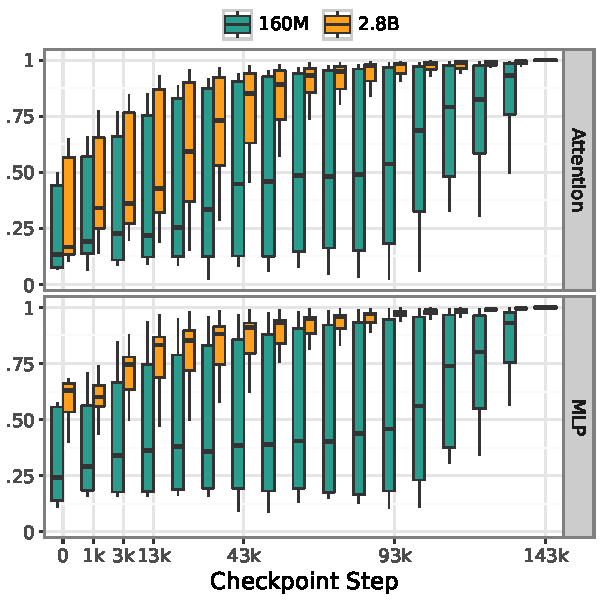
\includegraphics[width=0.58\columnwidth]{chapters/tending-towards-stability/figures/cka_main_plot.pdf}
    \caption{$\cka$ similarity (current vs.\ last checkpoint) of $\attention$ and $\mlp$ activations for Pythia \sixmil and \twobil. Distribution across layers: \integer{10}, \integer{25}, \integer{50}, \integer{75}, and \integer{90}-th percentiles per checkpoint.}
    \label{fig:cka_main_plot}
\end{wrapfigure}

Before presenting our detailed analyses, we briefly describe the structure of the main figures. \cref{fig:main-results} summarizes our core findings across three axes: (1) the convergence of activations as measured by $\cka$ similarity to final checkpoint activations (first column), (2) the proportional effective rank ($\per$) of layers' parameters (second column), and (3) the $\per$ of the corresponding parameter gradients (third column). Each row shows statistics for a different operation—$\attention$ (top) and $\mlp$ (bottom)—and each line represents the mean value across layers for five Pythia models ranging from 70M to 2.8B parameters.

In addition to these averaged results, \cref{fig:cka_main_plot} displays the inter-quartile range of $\cka$ similarity values averaged across layers for the smallest and largest models, and \cref{fig:cka-layer-wise-lines}, \cref{fig:per_weight-layer-wise-lines}, and \cref{fig:per_grad-layer-wise-lines} provide a layer-wise breakdown of convergence and rank dynamics (for both weights and gradients), respectively. These figures allow us to distinguish aggregate trends from layer-specific behaviors and to track how representational capacity and learning signals evolve during training.

\clearpage

\begin{figure*}[h!]
    \centering
    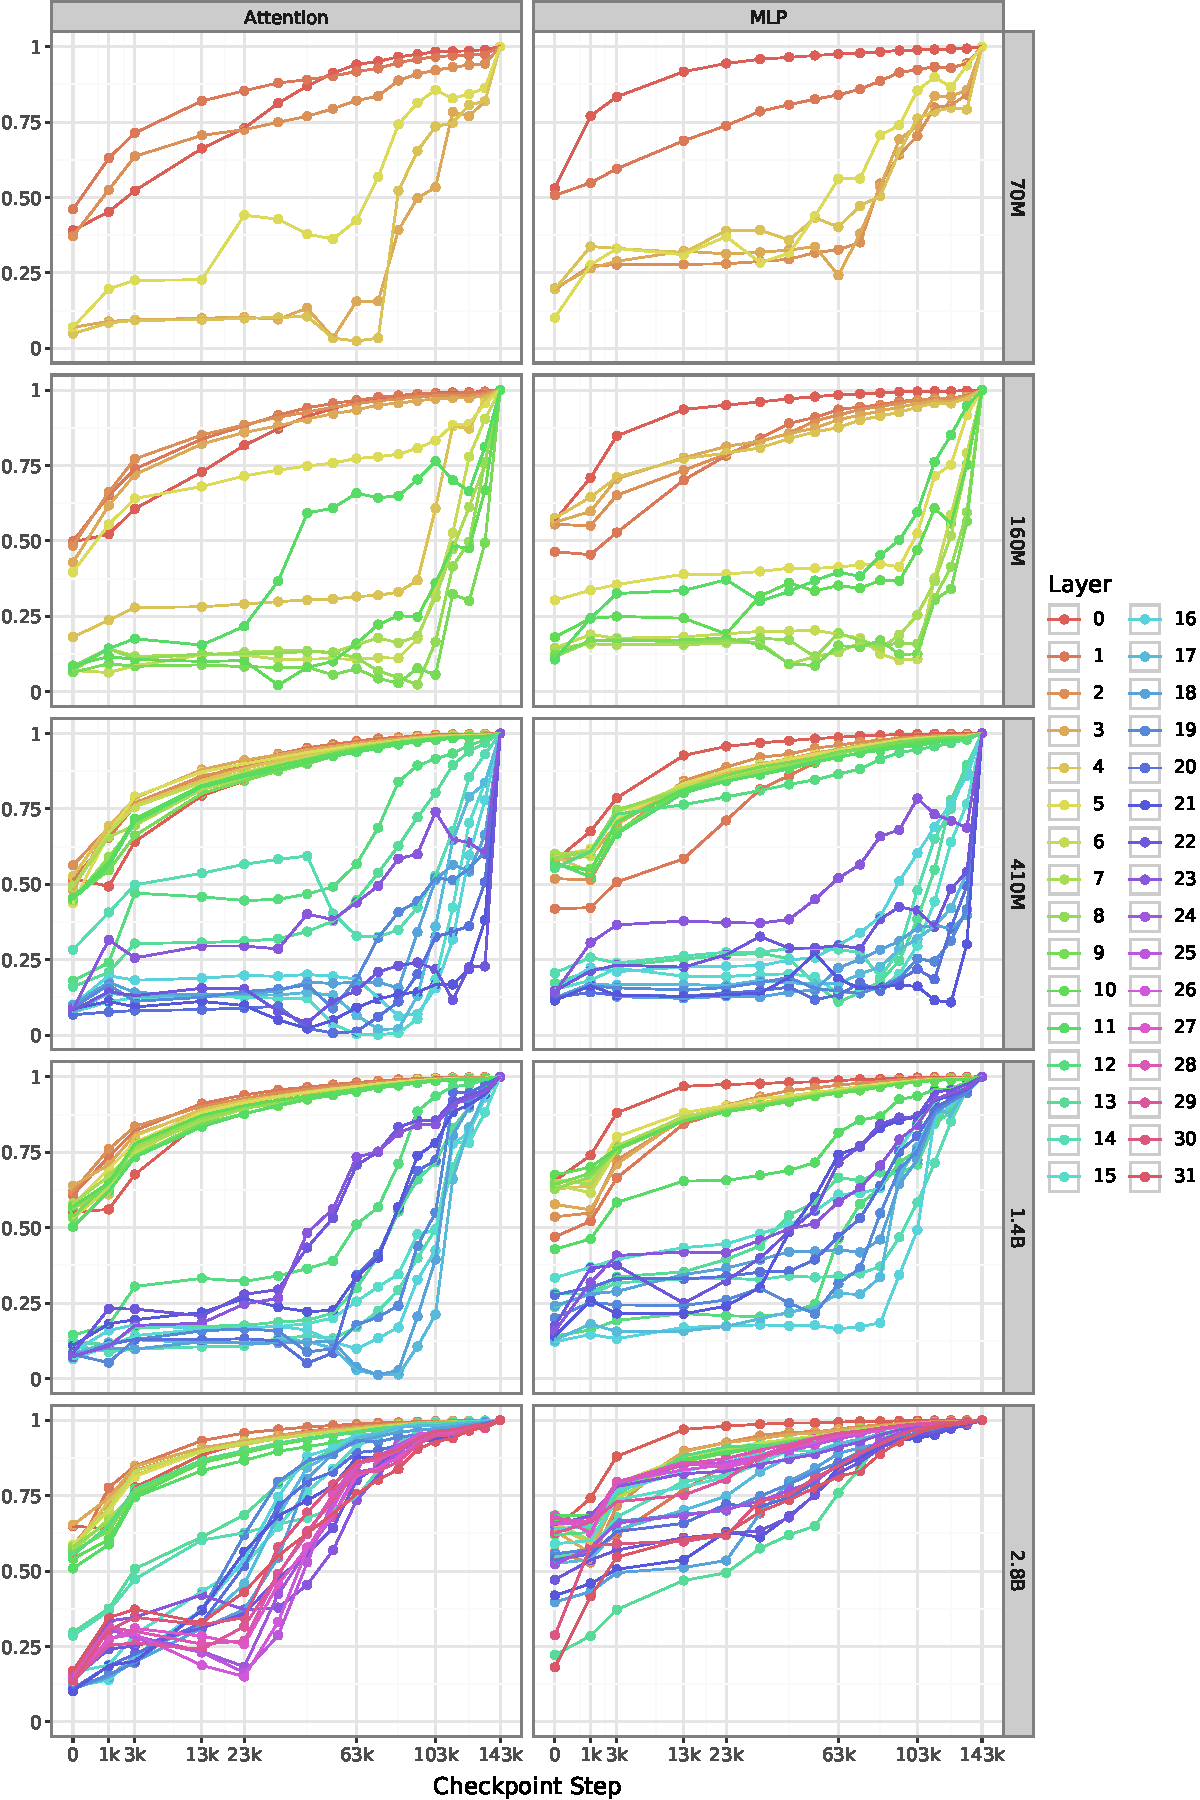
\includegraphics[width=0.9\linewidth]{chapters/tending-towards-stability/figures/cka_full_lines.pdf}
    \vspace{-5pt}
    \caption{$\cka$ similarity (current vs last checkpoint) of the activations of $\attention$ and $\mlp$ in each layer of Pythia \q{70}{\million}, \q{160}{\million}, \q{410}{\million}, \q{1.4}{\billion} and \q{2.8}{\billion} throughout training.}%
    \label{fig:cka-layer-wise-lines}
\end{figure*}
\clearpage

\begin{figure*}[h!]
    \centering
    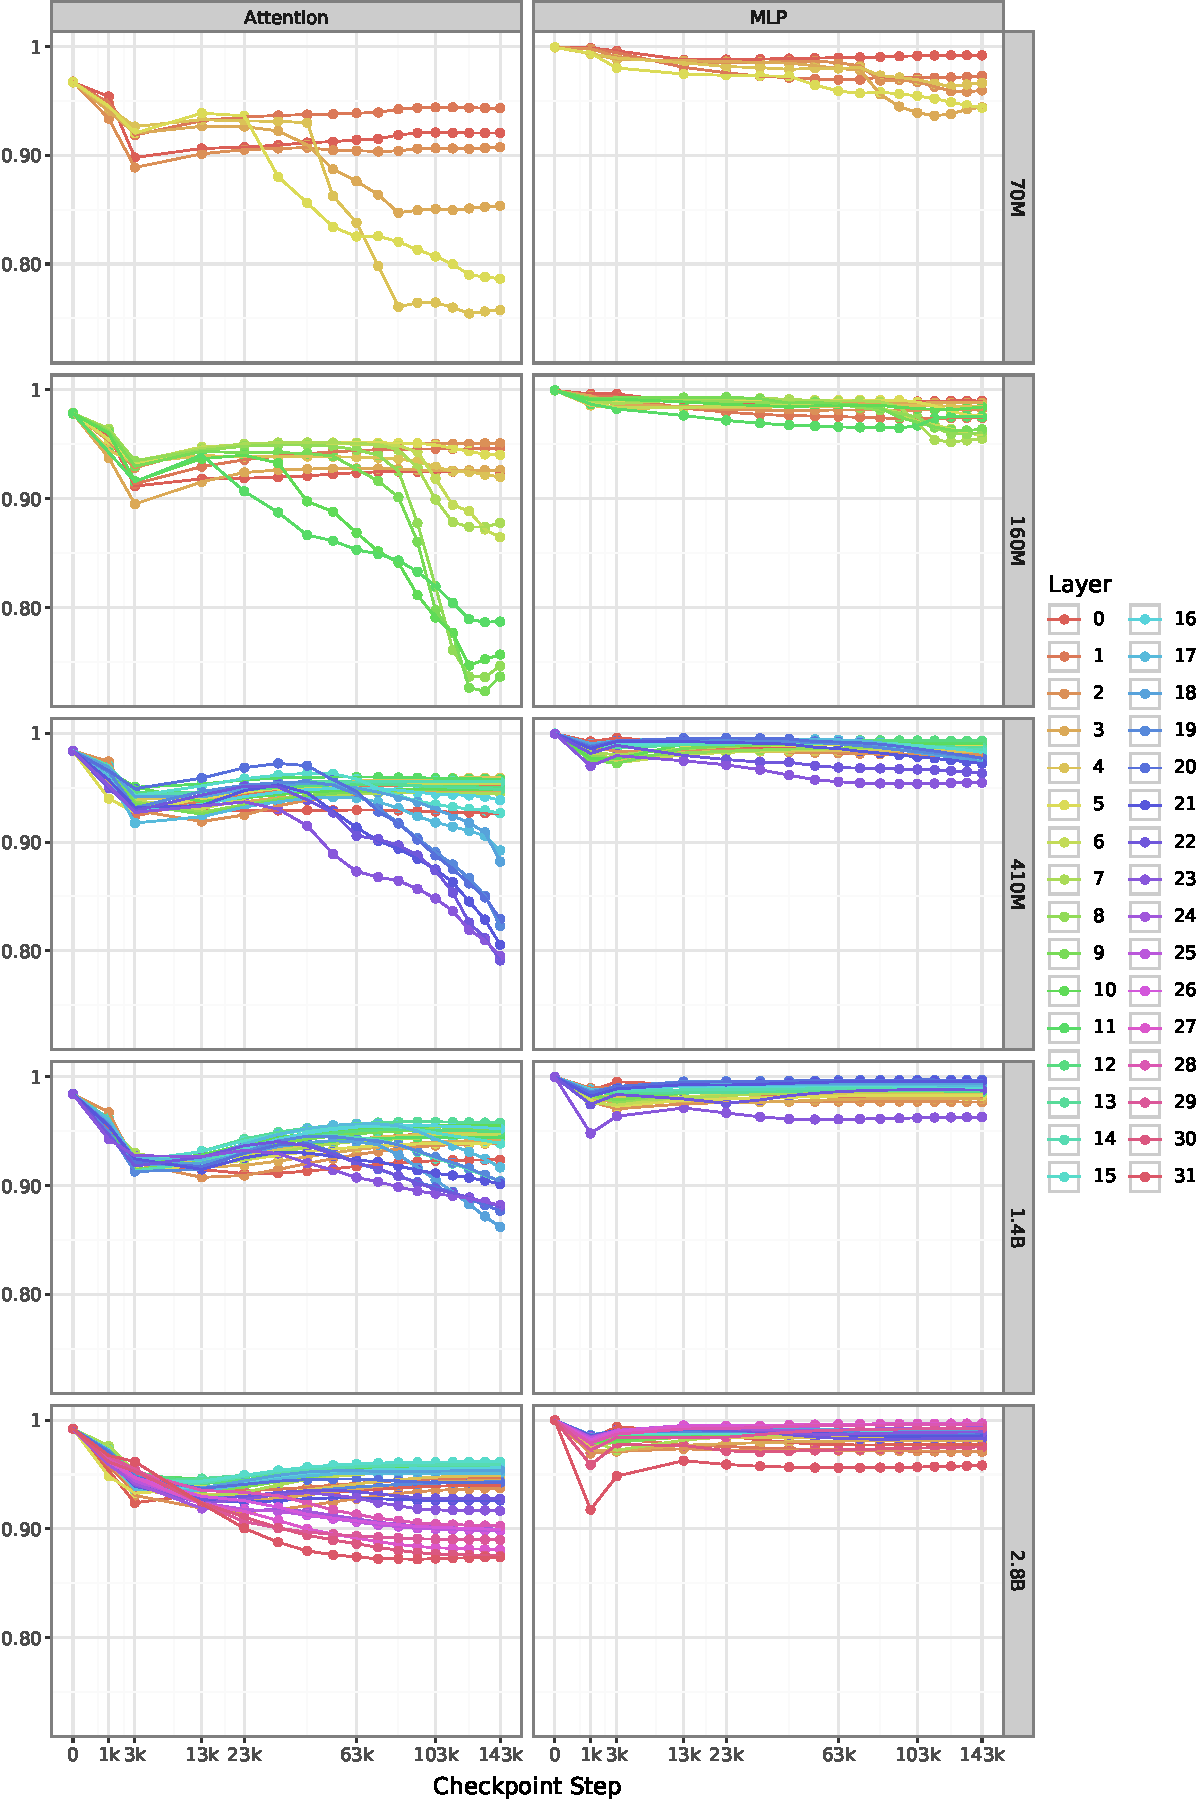
\includegraphics[width=0.9\linewidth]{chapters/tending-towards-stability/figures/per_weight_lines.pdf}
    \vspace{-5pt}
    \caption{$\per$ of the weight matrices of $\attention$ and $\mlp$ in each layer of Pythia \q{70}{\million}, \q{160}{\million}, \q{410}{\million}, \q{1.4}{\billion} and \q{2.8}{\billion} throughout training.}%
    \label{fig:per_weight-layer-wise-lines}
\end{figure*}
\clearpage

\begin{figure*}[h!]
    \centering
    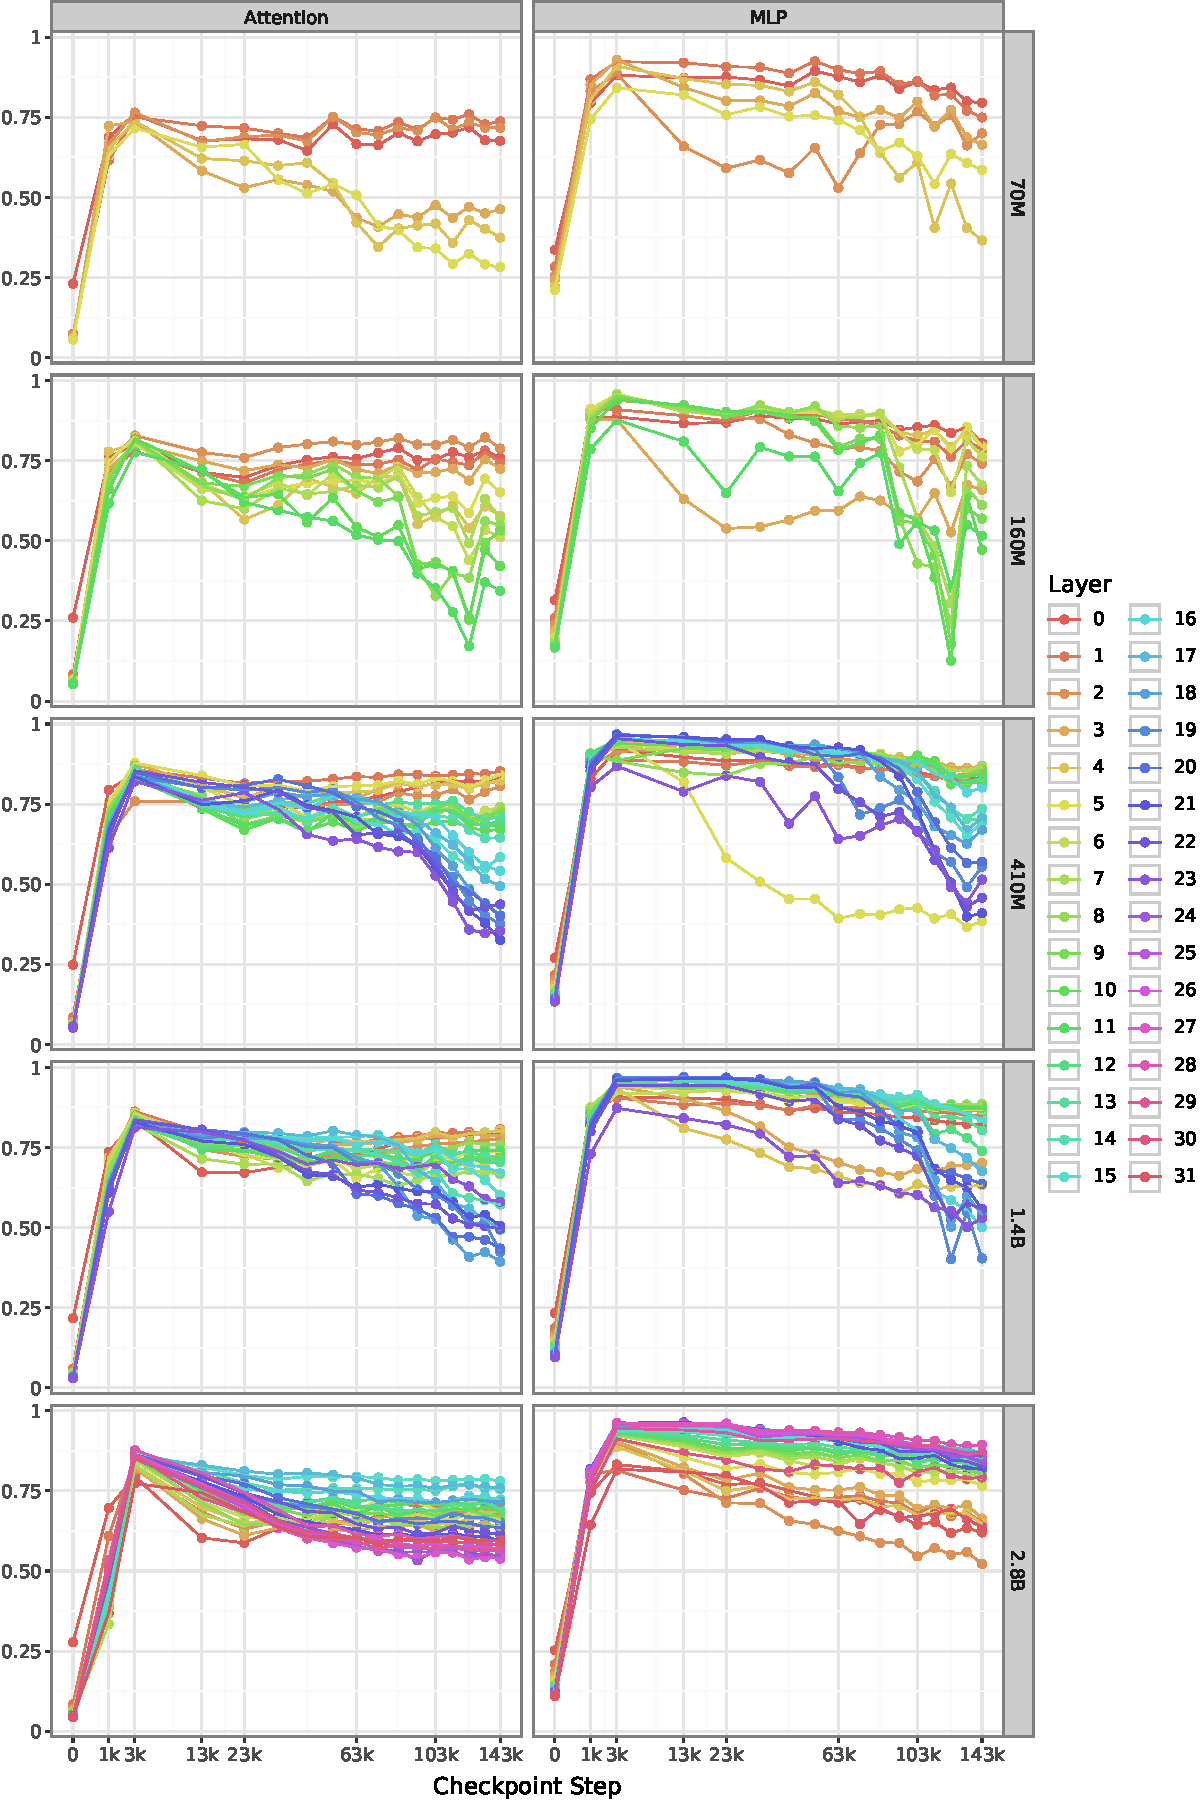
\includegraphics[width=0.9\linewidth]{chapters/tending-towards-stability/figures/per_grad_lines.pdf}
    \vspace{-5pt}
    \caption{$\per$ of the gradients of the weight matrices of $\attention$ and $\mlp$ in each layer of Pythia \q{70}{\million}, \q{160}{\million}, \q{410}{\million}, \q{1.4}{\billion} and \q{2.8}{\billion} throughout training.}%
    \label{fig:per_grad-layer-wise-lines}
\end{figure*}
\clearpage



\begin{result}[Activations of larger models converge faster and more monotonically to their final state than those of smaller models]
\label{result:cka}


As shown in the first column of \cref{fig:main-results}, $\cka$ similarity between a layer's activations at a given checkpoint and its final state rises more quickly in larger models. For instance, by 20\% of training, the $\cka$ score in \twobil reaches $\sim$0.8 for $\mlp$ and $\sim$0.7 for $\attention$, compared to values around 0.5 in \sevenmil and \sixmil. This trend reflects more rapid and stable convergence.

\cref{fig:cka_main_plot} adds further evidence: across checkpoints, the interquartile range (25th to 75th percentiles) of $\cka$ similarity across layers is both narrower and higher in larger models, confirming convergence is more uniform layer-wise.

\cref{fig:cka-layer-wise-lines} provides a more granular, layer-wise view: in \twobil, many layers—especially earlier ones—achieve high similarity early in training, whereas in smaller models convergence is delayed and less monotonic.

% As observed in \cref{fig:main-results} (first column), larger models show, on average, earlier convergence of $\attention$ and $\mlp$ activations. For example, by \q{20}{\percent} of training, the $\cka$ score in \twobil is \float[1]{0.8} for $\mlp$ and \float[1]{0.7} for $\attention$, where in \sevenmil and \sixmil it is around \float[1]{.5}.
% This fast convergence pattern holds across layers, as shown by the distributions in \cref{fig:cka_main_plot}.
\end{result}

\begin{result}[Activations of earlier layers converge faster, regardless of the model size]
Across model sizes, earlier layers' activations converge faster to their final state than those of later layers. As shown in \cref{fig:cka-layer-wise-lines}, the faster average convergence in larger models is due to more of their later layers converging earlier, whereas smaller models' layers only reach their final state towards the end of training.
\end{result}

\vspace{9pt}
Based on recent work that identifies parameter rank differences across model sizes \citep{godey2024small}, in the next paragraphs, we study whether the different convergence behaviours are related to the effective rank of layers' parameters and gradients.
\vspace{9pt}

\begin{result}[Parameters of layers in larger models proportionally span more dimensions] 
\label{result:weight-effective-rank} 
Parameters in layers of larger models span a slightly larger fraction of their available dimensions compared to smaller models, as shown in \cref{fig:main-results} (second column). 
Moreover, the $\per$ of larger models stabilises early, while it keeps decreasing throughout training for smaller ones. This finding is further underscored when visualising the $\per$ for each layer, as shown in \cref{fig:per_weight-layer-wise-lines}; we observe that in smaller models the $\per$ of later layers tends to decrease over the course of training, while in larger models the $\per$ of all layers stabilises early in training. This difference is even more pronounced in the $\per$ of these layers' gradients, as shown in \cref{fig:main-results} (third column).
\end{result}

\begin{result}[Parameters of layers in larger models receive gradient updates along proportionally more dimensions]
\label{result}
The $\per$ of gradients reflects the proportion of the learning signal transmitted by the gradients relative to the available parameter dimensions. In \cref{fig:main-results} (third column), we observe that throughout training gradients in larger models consistently span a larger fraction of the available dimensions, with this fraction gradually decreasing over time. In contrast, smaller models display more variability. At first glance, the averaged $\per$ of gradients in the $\attention$ layer of the \twobil model might appear to contradict the observed trend. However, this discrepancy is clarified when examining the $\per$ of gradients across individual layers, as shown in \cref{fig:per_grad-layer-wise-lines}. Once again, we observe that the $\per$ of gradients in later layers of smaller models are less stable compared to larger models. The reason the average $\per$ of gradients in the $\attention$ layer of the \twobil model is smaller than in smaller models is that, early in training, all layers of the larger model stabilise at their final values. At this stage, the stabilised layers of the larger model have lower gradient $\per$ values compared to those of smaller models, which have not yet converged. Overall, our findings suggest that layers in larger models converge both more quickly and tend to receive proportionally larger rank updates during training.
\end{result}


\begin{figure*}[h!]
    \centering
    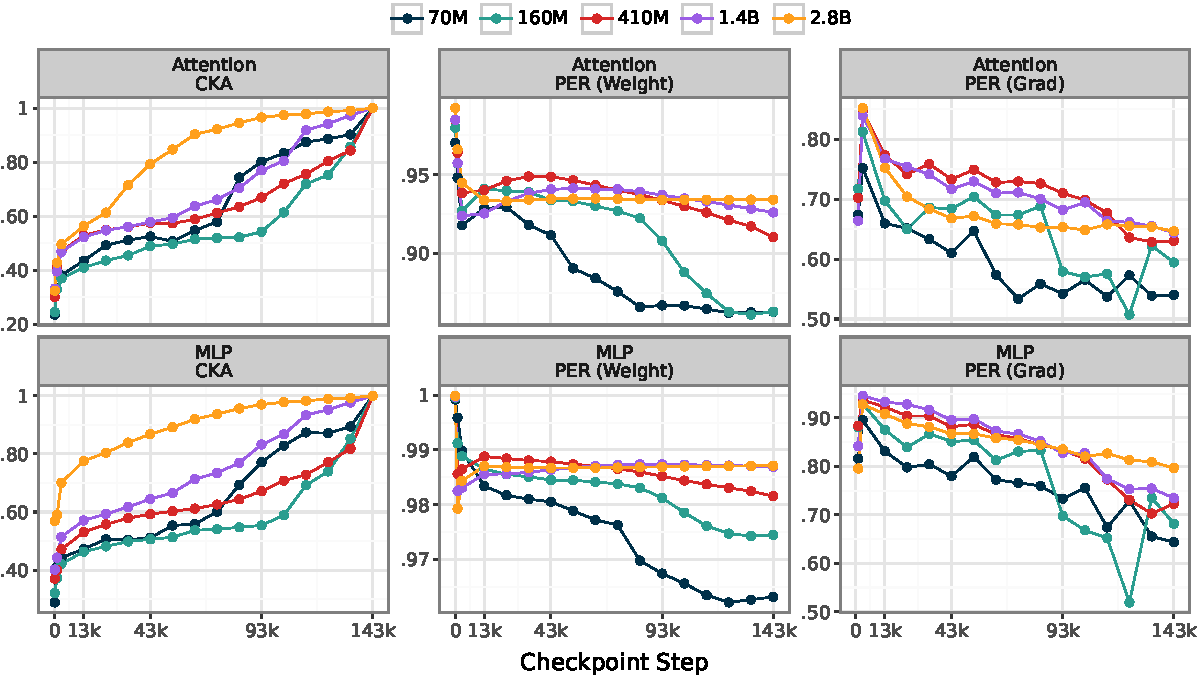
\includegraphics[width=\linewidth]{chapters/tending-towards-stability/figures/results.pdf}
    \vspace{-15pt}
    \caption{$\cka$ similarity (current vs.\ last checkpoint) of layers' activations (first column), $\per$ of layers' parameters (second column) and gradients (third column) for $\attention$ (top row) and $\mlp$ (bottom row) in Pythia \sevenmil, \sixmil, \fourmil, \onebil, and \twobil averaged (mean) across layers per each checkpoint.}
    \label{fig:main-results}
\end{figure*}


\begin{result}[The dynamics of the parameters' effective rank and the activations' convergence patterns are correlated]
We investigate the correlation between a layer's activations convergence rate and the rank of its parameters and gradients. Broadly, we find that layers with higher effective rank in both weights and gradients converge faster.
To measure this correlation, we first create two binary variables for each layer indicating whether (i) it converges early in training and (ii) maintains a stable $\per$ throughout training. Then, we calculate the Matthew's Correlation Coefficient between these two statistics across layers and report them in \cref{tab:model_correlation}.
Specifically, for each layer of a given model, we determine whether that layer exhibits early activations' convergence and large and stable parameters' and gradients' $\per$s (relative to other model layers) using the following heuristics: 
\begin{itemize}
    \item \textbf{Early activations' convergence.} Activations' $\cka \mathop{\geq} \float[2]{0.45}$ by the first \q{10}{\percent} of training (applies to both the $\attention$ and $\mlp$ layers).
    
    \item \textbf{Large parameters' $\per$.} Parameters' $\per \mathop{\geq} \float[2]{0.95}$ by the end of training (applies to both the $\attention$ and $\mlp$ layers).
    
    \item \textbf{Large gradients' $\per$.} We note that gradients' $\per$ slightly decreases throughout training for each model size. Rather than choosing a fixed value to determine large and stable gradients' $\per$s, we dynamically set the threshold at \q{90}{\percent} of the largest $\per$ attained by any layer at the end of training.
\end{itemize}
We observe a strong correlation for the $\attention$ layers across model sizes. For the $\mlp$ layers, the correlation with the gradients' $\per$ is strong for models up to \onebil, while the correlation with the parameters' $\per$ is strong only for the \sevenmil model. We hypothesize that this discrepancy can be explained by the fact that $\mlp$ layers have a large $\per$ throughout training across all model sizes, apart from those of the \sevenmil model. 

While these results are correlational, they provide a foundation for future work to test whether methods that specifically increase the PER of layers' parameters and gradients induce faster convergence of the layers' activations in small models.
\end{result}

\begin{table}[!t]
    \centering
    \begin{tabular}{crrrr}
\toprule
 \textbf{Size} & $\attweight$  & $\nabla \attweight$ & $\mlpweight$ & $\nabla\mlpweight$\\ 
\midrule
\sevenmil  & \float[2]{1.000} & \float[2]{1.000} & \float[2]{0.632} & \float[2]{1.00} \\ 
\sixmil & \float[2]{1.000} & \float[2]{0.845} & \float[2]{0.357} & \float[2]{0.714} \\ 
\fourmil & \float[2]{0.837} & \float[2]{0.916} & \float[2]{0.192} & \float[2]{0.777} \\ 
\onebil & \float[2]{0.775} & \float[2]{0.845} & \float[2]{0.209} & \float[2]{0.641} \\ 
\twobil & \float[2]{0.728} & \float[2]{0.521} & \float[2]{0.112} & \float[2]{0.179} \\ 
\bottomrule
\end{tabular}
    \caption{Matthew's Correlation Coefficient %($\phi$)
    between binary variables indicating whether a given layer converges early in training and whether it maintains a stable PER of the parameters ($\vtheta$) and gradients ($\nabla\vtheta$) throughout training for both $\attention$ and $\mlp$.}
    \label{tab:model_correlation}
\end{table}



% ===========
% CONCLUSIONS
% ===========
\section{Conclusion}

Our findings reveal consistent and interpretable distinctions in learning dynamics across model scales. Larger models exhibit faster and more monotonic convergence in their layer activations, and make fuller use of their representational capacity—evidenced by higher and more stable proportional effective ranks ($\per$) of both weights and gradients. In contrast, smaller models display delayed convergence, greater instability, and under-utilization of available capacity. These patterns suggest that part of the capability gap between small and large models may stem not from optimization failure per se, but from inefficient or truncated learning trajectories.

Importantly, these insights offer actionable hypotheses: for instance, that inducing higher-rank updates or more distributed gradient flows might help smaller models converge more like their larger counterparts. However, testing such hypotheses directly—by intervening on training dynamics and re-evaluating learning behavior—is difficult in practice.

Ideally, we would now like to modify the Pythia models—for example, to encourage higher effective rank early in training—and retrain them to see whether convergence patterns improve. Yet retraining Pythia is non-trivial. The framework poses several practical limitations:

\begin{itemize}[label=\xmark]
    \item \textbf{The dataset (The Pile)} is not easily streamable in its deduplicated format, and lacks a flexible preprocessing pipeline.
    \item \textbf{Training requires Megatron-DeepSpeed}, which introduces heavy engineering overhead, tightly coupled dependencies, and strict hardware requirements.
    \item \textbf{The models are distributed via Docker environments} with limited transparency, making it hard to debug, reproduce, or extend experiments.
    \item \textbf{Checkpointing and evaluation tools are fragmented or poorly documented}, complicating integration with analysis workflows.
\end{itemize}

To rigorously study learning dynamics—and in particular, to test targeted training interventions—we need a framework that makes model retraining as accessible as analysis. Such a framework should:

\begin{tcolorbox}[
    colback=white,
    colframe=thesisblue,
    title=\textbf{Design Requirements for Intervention-Friendly Language Model Platforms},
    fonttitle=\bfseries,
    coltitle=white,
    arc=0mm,
    boxrule=1pt,
    left=10pt,
    right=10pt,
    top=10pt,
    bottom=10pt,
    enhanced,
    breakable
]
To effectively support intervention-based research on language model training dynamics, an ideal platform should meet the following criteria:

\begin{itemize}[label=\cmark]
    \item \textbf{Transparency and Modularity}: Fully open-source with minimal external dependencies. Code should be clean, auditable, and modular to support rapid iteration and debugging.
    
    \item \textbf{Reproducible Training and Evaluation}: Provide ready-to-use scripts and configuration files for full training and evaluation pipelines. Baselines should be reproducible with minimal tuning.
    
    \item \textbf{Streamable and Standardized Data}: Support tokenized datasets in streaming formats with built-in preprocessing, packing, and filtering. Avoid proprietary dataset formats or brittle pipelines.
    
    \item \textbf{Intermediate Checkpointing}: Include well-timed checkpoints (e.g., log-spaced or per epoch) to track learning dynamics. Checkpoints should be saved in consistent formats and compatible with analysis tools.
    
    \item \textbf{Structured Logging}: Capture training statistics, gradients, and loss metrics in structured logs (e.g., JSONL, CSV) to enable downstream learning dynamics analysis.
    
    \item \textbf{Flexible Model Configuration}: Allow for easy experimentation with model size, layer depth, attention mechanisms, and other architectural choices through config files or flags.
    
    \item \textbf{Lightweight Hardware Requirements}: Be optimized for small and mid-sized models to enable training and analysis on affordable GPU setups, supporting high-velocity prototyping.
\end{itemize}
\end{tcolorbox}

These requirements motivate the development of the \pico model suite: a lightweight, transparent training and evaluation framework purpose-built for studying learning dynamics in small language models. In the next chapter, we introduce \pico and describe how it enables reproducible experiments on training dynamics, as well as targeted interventions to test and refine the hypotheses surfaced in this chapter.

